% Please do not change the document class
\documentclass{scrartcl}

% Please do not change these packages
\usepackage[hidelinks]{hyperref}
\usepackage[none]{hyphenat}
\usepackage{setspace}
\doublespace




% You may add additional packages here
\usepackage{amsmath}
\usepackage{cite}
\setlength{\parindent}{4em}
\usepackage{graphicx}

% Please include a clear, concise, and descriptive title
\title{Is Test-Driven Development Useful to Game Developers? 
A Case Study Exploring Applications to Data-Heavy Games}

% Please do not change the subtitle
\subtitle{COMP130 - Software Engineering}

% Please put your student number in the author field
\author{1703170}

\begin{document}

\maketitle

\textit{Test-driven development is becoming increasingly popular in the software engineering industry. It is professed by practitioners of test-driven development that it can improve code quality and maintainability and that automated tests can combat regression. However, there is a noticeable lack of the practice in the games industry. This paper explores the reasons behind this, as well as questioning how appropriate the practice is for data-heavy games.  }



\section*{Introduction}

There is much dispute in the games industry as to whether or not TDD is well suited for game development \cite{GameDev}\cite{GameDev2}. The purpose of this paper is to discuss the merits and weaknesses of TDD in a software engineering environment and how transferable these are to game development; with particular reference to its usefulness in data-heavy games such as The Sims 4 or Magic: The Gathering.



\section*{What is Test-Driven Development?}

Test-Driven Development (TDD) is an agile development practice \cite{beck2001manifesto}. It is essentially the act of writing tests for production code before writing enough production code to fulfill that test. If the tests fail then refactor until the tests pass and continue this cycle throughout the development process (see fig.1) \cite{beck2003test}.

There are a number of ways that programmers test and verify their code. Programmers can run the output to check if the application does what it's supposed to or manually check a program, using a debugger to step through code and verify it runs properly from the code base. The TDD way is to continuously create automatically running tests in parallel with production code to check that it is doing what the programmer wants.

\begin{center}
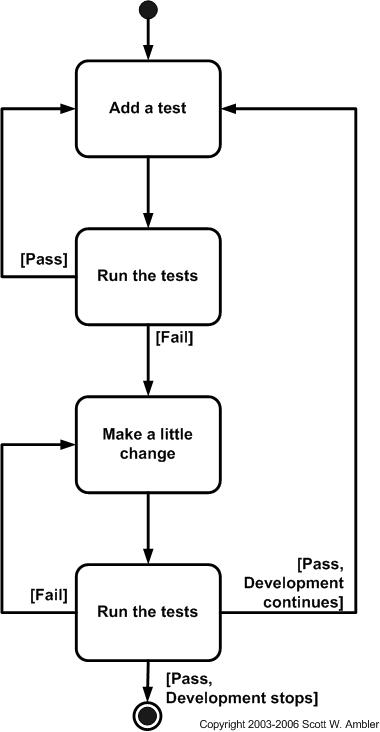
\includegraphics[scale=0.5]{tddSteps.png}
\end{center}

\begin{center}
\textit{Figure 1 - The basic steps of TDD}
\end{center}

\section*{The Merits of Test-Driven Development}

With traditional development methods, the process is as follows: design the program, implement the code, manually test the code. In this instance, manual testing is at the forefront of how a piece of software gets checked for bugs. This does however have it's drawbacks. For example, this manual testing will need to occur at the end of the implementation phase of every feature added to the program. This is fine for small programs, however the bigger a project becomes the more features are added. For every new feature, the likelyhood that another piece of code is adversely affected increases (regression defects affecting existing functionality). More testing is required to find and fix new bugs, thus lengthening development time and cost exponentially \cite{boehm1981software} (see fig.2). Studies show us that developers use on average 30-40 percent more effort than is initially estimated at the start of a  project \cite{jorgensen2007systematic}. With more agile iterative development techniques such as TDD, the cost in development can be significantly lessened, making more frequent testing far more feasible. Theoretically, TDD can flatten out the cost of change curve in the long run in exchange for a slightly more costly set up cost at the start of development \cite{GDCBackwards} (see fig.3). This trade-off is more substantial with larger teams and more complex systems for obvious reasons. A study at IBM is an example of the reduction in the risk of regression defects with the use of TDD compared to other approaches \cite{williams2003test}. A project using TDD can be far more maintainable and changeable later on nearer the end of development. 



Another benefit to TDD is how it affects the psychological welfare of the programming team. Often programmers in a team taking a more traditional approach to development may go weeks without feedback on large features or even months depending on sprint lengths. When a features is finally tested it is  likely to contain significant bugs or have created problems with other features. With TDD however,  through the constant use of small automated unit tests, the programmer receives regular positive feedback in the form of their code passing these tests \cite{GamaEmbracingFun}. Of course this assumes that the tests will generally pass, but even when they don't they should be caught quickly, thus making the next set of tests more likely to pass than not. This can boost the morale of the programmers writing the code and keep the team as a whole more energised \cite{GDCBackwards}.




\begin{center}
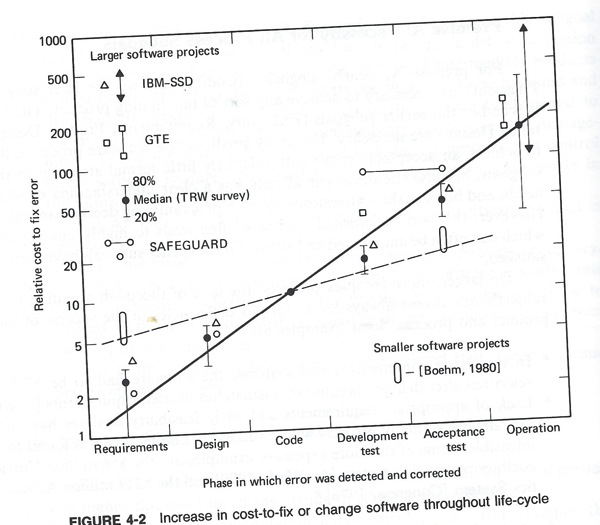
\includegraphics[scale=0.4]{costofchange.png}
\end{center}

\begin{center}
\textit{Figure 2 - Barry Boehm's original Cost of Change Curve }
\end{center}

\begin{center}
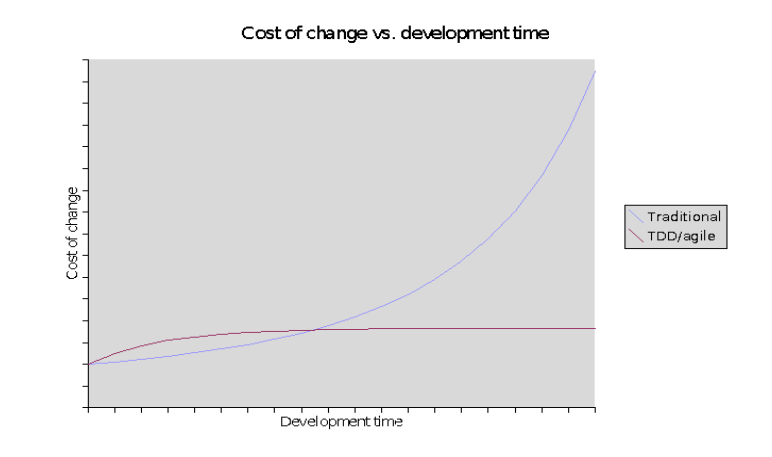
\includegraphics[scale=0.6]{newcostofchange.png}
\end{center}

\begin{center}
\textit{Figure 3 - Ideal Cost of Change Curve with TDD vs Traditional}
\end{center}

\section*{The Weaknesses of Test-Driven Development}

As previously discussed, it has been shown that TDD can save a company time and money with regards to catching bugs much earlier and more frequently \cite{kayongo2016software} \cite{GDCBackwards}. However there is continued debate, particularly in the games industry, as to whether or not the time saved in the manual testing phase of development is outweighed by the extra cost in time it takes to write the extra code in the form of automated unit tests\cite{stackover}. Some programmers in studies have expressed concerns about this increase in development time that is required to write unit tests \cite{george2003initial}.  

It is possible that in companies where TDD fails there are other considerations to be made as to why this is. Some programmers fail to understand what TDD is \cite{janzen2008does} and it is not unreasonable to suggest that programmers new to TDD will be much less productive when first adapting to the process. There are studies that support the idea that programmers feel like it is difficult to get into the TDD mindset \cite{george2003initial}. This suggests it may be beneficial for development teams new to TDD to start on a small scale perhaps with pair programming with individuals with prior TDD experience. This may be why most large game development companies choose to not take the risk in implementing TDD as these possible weaknesses are a cause for concern for game companies.


\section*{Test-Driven Game Development}

There is much debate in the games industry as to whether TDD is useful to game developers. Some consider TDD to be less helpful when developing games, suggesting that \textquotedblleft we cannot test fun". This possibly misses the point that advocates of TDD make however. The usefulness of TDD to game development lies, not in the testing of how a game plays, but in the maintainability of the architecture and good code practice \cite{UncleBob}. There is also good reason to think that TDD can benefit smaller teams that don't have the vast resources and quality assurance departments that AAA companies have. One reason is that having a stable game can free up the designer to experiment with the gameplay more to \textquotedblleft find the fun" without programmer intervention\cite{GamaTDDExp}. This boon can be invaluable to a small development team.

Automated unit tests in games development can be critical to fighting hidden regression \cite{GamaEmbracingFun} and would be well suited to testing the functionality of game code. Automated unit tests, which are a fundamental aspect of TDD, can be used in game engines to check physics, geometry, rendering, network logic, game settings etc. Therefore, although a development team cannot rely solely on TDD for some aspects of game design - such as the usability, feel, style and aesthetics that make the game an enjoyable experience - TDD can offer much in the way of keeping the core functionality of the game systems working. 

TDD may be more useful in the development of certain types of games. Data-Heavy games face a particular issue in regards to generating overwhelming code complexity. This is evidenced in the making of the Sims 4 \cite{GDCConcurrent}. With this game, the developers needed to build a multitasking system with certain constraints to dictate if, when and how the Sim would be able to interact with multiple objects. This is a system with less tolerance for ad-hoc implementation and so anything to help with reducing code complexity and aid continuous integration is a boon to designers.  As previously discussed, TDD is an ideal fit for alleviating code complexity and encourages code simplicity \cite{amrit2017effectiveness}. Automated unit tests would be especially useful given the vast number of data-driven tasks and constraints concurrent interactions require. 

TDD would therefore clearly be useful in games that continue development after release. Games like Duel Links or Magic: The Gathering are card games that continually release new content with new cards that have new interactions with already implemented cards. With TDD, a programmer is more safe in the knowledge that regression is less likely and previous features are better guarded with automated tests \cite{GDCBackwards}. As a general rule, low-level code that other code will depend on is well suited to unit testing\cite{GDCBackwards}. This makes maintaining a code base and adding new features that interact with the code much less complex and far easier and quicker to do. This simplification of the code can streamline more Data-Heavy games to a certain extent.

 



\section*{Limitations}

There are limitations to this paper. TDD is not widely used in the games industry, this means test cases specific to games have been difficult to source. High Moon Studios is the only game studio that is referenced in this paper and as such most of my findings are inferences based on papers dealing with TDD in general software engineering or grey literature on discussions on the usefulness of TDD in games. 

\section*{Conclusion}

In conclusion, opinion is divided. The practices of TDD can be useful to game developers, but how strictly the rules of TDD are followed \cite{UncleBob} and how useful they are is dependent on the type of game being made and the priorities of the developers. The best practices in the game industry tend to use similar techniques to those in TDD to reap the same benefits \cite{fucci2017dissection} without the extra initial time sink and learning curve, and so TDD can sometimes be seen as an unnecessary annoyance, at least initially. More corporate AAA game companies have large Quality Assurance departments, so the benefits of automated unit tests can be negated to a certain extent. Also, TDD appears to be well suited to games with complex functional interactions because unit test are well suited to testing functionality \cite{GDCConcurrent}. 

From the findings of this paper, it can be inferred that there is a chance TDD will become more widely used in the industry due to the advent of more 'games as a service' games with continuous development routes, as TDD goes hand with Continuous Integration which is useful for these types of games. However, until more game companies start using TDD, this is difficult to test and is mainly speculation.




\bibliographystyle{ieeetran}
\bibliography{references}

\end{document}




